\documentclass{article}


% if you need to pass options to natbib, use, e.g.:
\PassOptionsToPackage{numbers, sort&compress}{natbib}
% before loading neurips_2022


% ready for submission
\usepackage{neurips_2022}

% to compile a preprint version, e.g., for submission to arXiv, add add the
% [preprint] option:
%     \usepackage[preprint]{neurips_2022}


% to compile a camera-ready version, add the [final] option, e.g.:
%     \usepackage[final]{neurips_2022}


% to avoid loading the natbib package, add option nonatbib:
% \usepackage[nonatbib]{neurips_2022}


\usepackage[utf8]{inputenc} % allow utf-8 input
\usepackage[T1]{fontenc}    % use 8-bit T1 fonts
\usepackage{hyperref}
% \usepackage{subfigure}
\usepackage{graphicx}    % hyperlinks
\usepackage{url}            % simple URL typesetting
\usepackage{color}
\usepackage{booktabs}       % professional-quality tables
\usepackage{amsfonts}       % blackboard math symbols
\usepackage{nicefrac}       % compact symbols for 1/2, etc.
\usepackage{microtype}      % microtypography
\usepackage{xcolor}         % colors
\usepackage{wrapfig}


\usepackage{times}
\usepackage{epsfig}
\usepackage{amsmath}
\usepackage{amssymb}

% Include other packages here, before hyperref.
\usepackage{float}
\usepackage{bbding}
\usepackage{pifont}
\usepackage{wasysym}
\usepackage{multirow}
\usepackage{subfig}



\title{Self-Supervised Spatial-Temporal Feature Learning for Video Correspondence \\
----- NeurIPS 2022 Supplementary Material}


% The \author macro works with any number of authors. There are two commands
% used to separate the names and addresses of multiple authors: \And and \AND.
%
% Using \And between authors leaves it to LaTeX to determine where to break the
% lines. Using \AND forces a line break at that point. So, if LaTeX puts 3 of 4
% authors names on the first line, and the last on the second line, try using
% \AND instead of \And before the third author name.

\author{%
  David S.~Hippocampus\thanks{Use footnote for providing further information
    about author (webpage, alternative address)---\emph{not} for acknowledging
    funding agencies.} \\
  Department of Computer Science\\
  Cranberry-Lemon University\\
  Pittsburgh, PA 15213 \\
  \texttt{hippo@cs.cranberry-lemon.edu} \\
  % examples of more authors
  % \And
  % Coauthor \\
  % Affiliation \\
  % Address \\
  % \texttt{email} \\
  % \AND
  % Coauthor \\
  % Affiliation \\
  % Address \\
  % \texttt{email} \\
  % \And
  % Coauthor \\
  % Affiliation \\
  % Address \\
  % \texttt{email} \\
  % \And
  % Coauthor \\
  % Affiliation \\
  % Address \\
  % \texttt{email} \\
}


\begin{document}


\maketitle

The supplementary material contains:  1) ablation study of different contrastive models; 2) ablation study of entropy-based selection;  3) more qualitative examples for video object segmentation.

\section{Ablation study of different contrastive models}
Given a query point randomly sampled in the target frame, we visualize the result of computing the local correlation and global correlation map $w.r.t.$ reference frame. The dashed line in red represents the range of computing correlation map $w.r.t.$ query point. The reference frame is randomly sampled in the memory  bank of inference strategy. Given a query point randomly sampled in the target frame, we visualize the result of computing the local correlation and global correlation map $w.r.t.$ reference frame. The dashed line in red represents the range of computing correlation map $w.r.t.$ query point. The reference frame is randomly sampled in the memory  bank of inference strategy.Given a query point randomly sampled in the target frame, we visualize the result of computing the local correlation and global correlation map $w.r.t.$ reference frame. The dashed line in red represents the range of computing correlation map $w.r.t.$ query point. The reference frame is randomly sampled in the memory  bank of inference strategy

\section{Ablation study of entropy-based selection}
\begin{wraptable}{r}{6.5cm}
	\centering
	\small
	\resizebox{0.4\textwidth}{!}{
			\setlength\tabcolsep{10pt}
		\renewcommand\arraystretch{1.05}
    \begin{tabular}{@{}cccc@{}}
      \hline
      Method         & Dataset       &$\mathcal{J} \& \mathcal{F}_m \uparrow$ \\ 
      \hline
      T = 0.1 &  YTV    &67.4          \\
      T = 0.4 &  YTV    &68.3          \\
      T = 0.7    & YTV  &69.0          \\
      % + EWC            & ImageNet & Res50 &68.9          \\
      T = 1.0     & YTV  &68.1          \\
      \hline
    \end{tabular}%
	}
	\captionsetup{font=small}
	\caption{\textbf{The quantitative results on the validation set of DAVIS-2017.} The Dataset represents dataset(s) used for training. YTV:YouTube-VOS~\cite{}}
	\label{table:supp_en}
	\vspace{-5pt}
\end{wraptable}
We make detailed ablation study for our entropy-based selection in terms of both visual perception and quantitative comparison. As shown in Figure \ref{fig:supp_en}, the entropy map has a higher response on moving objects involved in severe deformation and occlusions, which should be paid more attention to. In Table ~\ref{table:supp_en}, we adopt different thresholds to generate the mask $m$ with high entropy. The baseline is to apply local correlation distillation for all queries, $i.e.$, T = 1.0. When setting T with 0.1, the performance drops to 67.4\% due to the underutilization of the supervision from finest pyramid level. The results of setting T with 0.4 and 0.7 indicate applying distillation in the region with high entropy exhibits a performance gain.
\begin{figure}[t]
  \centering
  {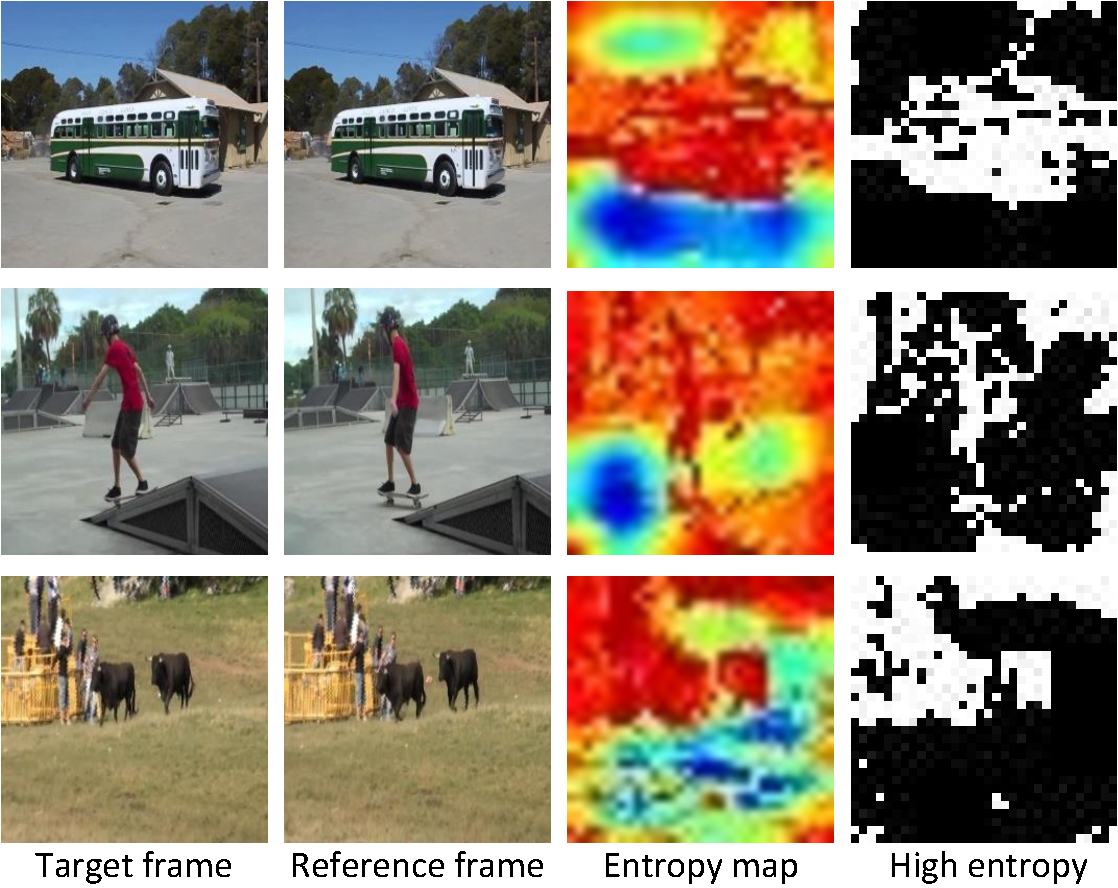
\includegraphics[width=0.6\textwidth]{figure/supp_entropy/supp_en.pdf}}
  \caption{\small \textbf{Visualization of the entropy map.} We compute the entropy for each query in target frame using Eq \textcolor{red}{8} in our main paper. The mask with high entropy is generated by setting a threshold. }
  \label{fig:supp_en}
  \vspace{-1mm}
\end{figure}

% \begin{table*}[b]
% \centering
% \begin{tabular}{@{}cccc@{}}
%   \hline
%   Method         & Dataset       &$\mathcal{J} \& \mathcal{F}_m \uparrow$ \\ 
%   \hline
%   T = 0.1 &  YTV    &67.4          \\
%   T = 0.4 &  YTV    &68.3          \\
%   T = 0.7    & YTV  &69.0          \\
%   % + EWC            & ImageNet & Res50 &68.9          \\
%   T = 1.0     & YTV  &68.1          \\
%   \hline
% \end{tabular}%
% \caption{\small The quantitative results of setting different thresholds.}
% \label{tab:supp_en}
% \end{table*}


\section{More qualitative examples for video object segmentation}
We do the most of experiments



\end{document}